\section{Perception Challenge}

\subsection{Challenge definition}

The perception challenge is titled "Thimblerigger". An iCUB robot starts in an empty world that contains three red cylinders. A cylinder represents a mug.
One of these mugs contains a green ball underneath. The challenge can reveal which mug contains the ball on request.
The task is to enable the robot to: 
\begin{enumerate}
	\item Find the mug that contains the ball
	\item Track that mug while the mugs are being shuffled
	\item Decide which mug contains the ball after shuffling
\end{enumerate}

Fig.~\ref{fig:challenge} displays the setup of the challenge.

\begin{figure}
	\centering
	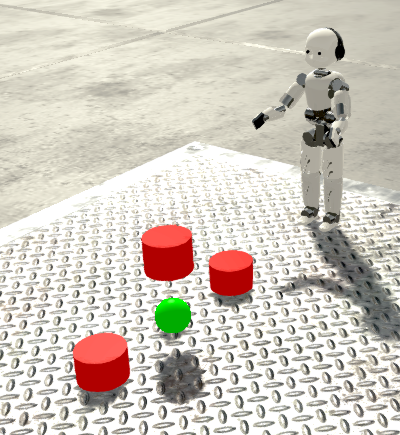
\includegraphics[width=0.4\textwidth]{logos/challenge}
	\caption{The perception challenge environment. The 	second mug is lifted up to display that it contains the 	ball.}
	\label{fig:challenge}
\end{figure}

In the following, we describe approaches to solve the challenge.

\subsection{Working version}

We solve the challenge via a distance-based approach. We move the robot to capture the scene from the side instead of from the front to avoid overlapping mugs in the camera image stream.

We employ four transfer functions to track the ball:
\begin{enumerate}

	\item Track green: Maps the green channel of the input image stream to three neurons $green_i, i\in\{1,2,3\}$. 
	\item Find initial track: Notices once the correct mug is lifted at challenge start by observing the output spikes of  $green_i, i\in\{1,2,3\}$.
	\item Extract centers: Finds the positions of all three mugs in frame $t$ by finding the center points of the three most prominent red contours in the input image stream. For this reason it is important that the mugs do not overlap themselves in the input image stream. The transfer function keeps track of the center point of the predicted mug in frame $t-1$. The prediction is updated based on the closest distance of the previous prediction to the current centers.
	\item Predict: Maps the mug index predicted to contain the ball to one of three $estimate_i,  i\in\{1,2,3\}$ neurons.
\end{enumerate}

All transfer functions requiring image input from the robot camera rely on the stream from the "left eye" camera. Equations~\eqref{eq:distance0} to \eqref{eq:distance10} formalize the tracking mechanism.

In equation~\eqref{eq:distance0}, we define the amplitude of the $green$ neurons  responsible for tracking the green ball to be the mean value of the green channel $g$ in their respective third at time $t$.
\begin{equation}
amplitude(green_{i_t}) = \begin{bmatrix}
           \frac{1}{93}\sum\limits_{y=120}^{160}\sum\limits_{x=85}^{137}g(x+y) \\
           \frac{1}{93}\sum\limits_{y=120}^{160}\sum\limits_{x=138}^{191}g(x+y) \\
           \frac{1}{92}\sum\limits_{y=120}^{160}\sum\limits_{x=192}^{240}g(x+y) \\
         \end{bmatrix}_{i_t}  \label{eq:distance0}
\end{equation}
       
Equations~\eqref{eq:distance2} through \eqref{eq:distance6} describe how the center points of the mugs are extracted from the input image stream. Here, $f$ is a manually tuned threshold function, $r$ is the red channel of the input image, and $b$ is a structuring element defined over $B$ such that $(b \ominus f)$ implements morphological erosion. $C$ is set of $(x,y)$ coordinates of contour center points in the eroded image ordered by their $x$ coordinate.
\begin{align}
f(x) &= \mathbbm{1}\{x >= 150\}\label{eq:distance2}\\
(b \ominus f)(x) &= \inf\limits_{y\in B}[f(x+y)-b(y)]\\
C_{outlines} &= \{c \in contours((b \ominus f)(x)): area(c) > 50\}\\
C &= \{center(c): x \in C_{outlines}\}_{\leq (x,y)}\label{eq:distance6}\\
\end{align}
Finally, $E_{t}$ is the estimated mug index at time $t$. Time $t=0$ is defined to be the moment a $green$ neuron spikes for the first time. The rate of the estimate neuron corresponding to the currently estimated index is set to $100$.
\begin{align}
E_0 &= \argmax\limits_i green_{i_0} \\ 
E_{t} &= \argmin\limits_{i}||C_i - E_{t-1}||_2 \\
rate(estimate_{i, i\in\{1,2,3\}, i\neq E_{t}}) &= 0 \\
rate(estimate_{E_{t}}) &= 100 
\label{eq:distance10}
\end{align}

Using this approach, the challenge is solved close to 100\% of trials. It only fails if a glitch occurs inside the simulator during repositioning of the robot, causing it to fall over. This happens in about $\frac{1}{40}$ of trials and is presumably caused by a race condition inside Gazebo, although this could not be verified.




\subsection{Other approaches}

Two approaches that utilize the spiking neural network to a higher degree have been tested. However, none of them worked to our satisfaction for different reasons. The following paragraphs describe the approaches and why we believe they fail.
